%----------------------------------------------------------------------------------------
%	PACKAGES AND OTHER DOCUMENT CONFIGURATIONS
%----------------------------------------------------------------------------------------

\documentclass[paper=a4, fontsize=11pt]{scrartcl} % A4 paper and 11pt font size

\usepackage[T1]{fontenc} % Use 8-bit encoding that has 256 glyphs
%\usepackage{fourier} % Use the Adobe Utopia font for the document - comment this line to return to the LaTeX default
\usepackage[english]{babel} % English language/hyphenation
\usepackage{amsmath,amsfonts,amsthm} % Math packages
\usepackage{graphicx}
\usepackage{listings}
\usepackage{color}

\definecolor{dkgreen}{rgb}{0,0.6,0}
\definecolor{gray}{rgb}{0.5,0.5,0.5}
\definecolor{mauve}{rgb}{0.58,0,0.82}

\lstset{frame=tb,
  language=python,
  aboveskip=3mm,
  belowskip=3mm,
  showstringspaces=false,
  columns=flexible,
  basicstyle={\small\ttfamily},
  numbers=none,
  numberstyle=\tiny\color{gray},
  keywordstyle=\color{blue},
  commentstyle=\color{dkgreen},
  stringstyle=\color{mauve},
  breaklines=true,
  breakatwhitespace=true,
  tabsize=3
}
%\usepackage{lipsum} % Used for inserting dummy 'Lorem ipsum' text into the template

\usepackage{sectsty} % Allows customizing section commands
%\allsectionsfont{\centering \normalfont\scshape} % Make all sections centered, the default font and small caps

\usepackage{fancyhdr} % Custom headers and footers
\pagestyle{fancyplain} % Makes all pages in the document conform to the custom headers and footers
\fancyhead{} % No page header - if you want one, create it in the same way as the footers below
\fancyfoot[L]{} % Empty left footer
\fancyfoot[C]{} % Empty center footer
\fancyfoot[R]{\thepage} % Page numbering for right footer
\renewcommand{\headrulewidth}{0pt} % Remove header underlines
\renewcommand{\footrulewidth}{0pt} % Remove footer underlines
\setlength{\headheight}{13.6pt} % Customize the height of the header

\numberwithin{equation}{section} % Number equations within sections (i.e. 1.1, 1.2, 2.1, 2.2 instead of 1, 2, 3, 4)
\numberwithin{figure}{section} % Number figures within sections (i.e. 1.1, 1.2, 2.1, 2.2 instead of 1, 2, 3, 4)
\numberwithin{table}{section} % Number tables within sections (i.e. 1.1, 1.2, 2.1, 2.2 instead of 1, 2, 3, 4)

%\setlength\parindent{0pt} % Removes all indentation from paragraphs - comment this line for an assignment with lots of text

%----------------------------------------------------------------------------------------
%	TITLE SECTION
%----------------------------------------------------------------------------------------

\newcommand{\horrule}[1]{\rule{\linewidth}{#1}} % Create horizontal rule command with 1 argument of height

\title{	
\normalfont \normalsize 
\textsc{Stanford CS 229 Fall 2017} \\ [25pt] % Your university, school and/or department name(s)
\horrule{0.5pt} \\[0.4cm] % Thin top horizontal rule
\Large Final Project Milestone: \\
\Large Real Time Tennis Match Prediction Using Machine Learning\\ % The assignment title
\horrule{2pt} \\[0.5cm] % Thick bottom horizontal rule
}

\author{Yang "Eddie" Chen, Yi Zhong, Yubo Tian} % Your name

\date{\normalsize\today} % Today's date or a custom date

\begin{document}

\maketitle % Print the title

%----------------------------------------------------------------------------------------
%	Section 1 Motivation
%----------------------------------------------------------------------------------------

\section{Motivation}
In the 2017 Stuttgart Open, Roger Federer, then an 18-time grand slam champion, lost to the world No. 302 player Tommy Haas on a grass court, which hadn't happened since 2002.  Based on past performance alone, any model would have predicted a Federer win in pre-game bets. This motivates us to apply machine learning to predict tennis matches in real time; in particular, we want to apply a hybrid model that combines historical and real-time information, similar to the model used by ESPN in-game prediction for NFL games.

Tennis is an ideal candidate for using a hierarchical probability model as a match consists of a sequence of sets, which in turn consist of a sequence of games, which in turn consist of a sequence of points.  Recent researches also began to apply machine learning on tennis pre-game predictions based on past performance (including previous encounter, current ranking, etc). Utilizing existing data and building on top of existing research such as Sipko \cite{tennis1}, Clarke and Dyte \cite{Clarke2010} and Knottenbelt \cite{KNOTTENBELT20123820}, this paper seeks to apply classification algorithms from machine learning to model men's professional singles matches by using both pre-game, historical performance calcualted via a common opponent model \cite{KNOTTENBELT20123820}, and real-time, on-court stats \cite{tennis_charting} \cite{tennis2setbyset}. As pointed out by Sipko \cite{tennis1}, an in-game approach "allows the model to capture the change in a player's performance over the course of the match. For example, different players fatigue during a match in different ways." We hope that results from our predictions can be extended to give real-time coaching advice to support game strategy decision.
%----------------------------------------------------------------------------------------
%	Section 2 - Method
%----------------------------------------------------------------------------------------

\section{Method}
\subsection{Feature Extraction}
\subsubsection{Feature Representation}
\label{sec:label}
Each training example contains features from historical and real-time aspect.  For the scope of this project, real-time aspect will be defined as the performance in previous set, as time information is not available from our dataset:
\begin{enumerate}
\item A vector of input features (X), describing the historical performance of both players and performance in previous set
\item A target value (y), indicating the match outcome
\end{enumerate}
In any given singles match, we have two players in one game. We denote them as Player 1 and Player 2, and thus define the target value as 
$y = 1$ if Player 1 wins, 0 otherwise. In the datasets we found online, it is usually the case that Player 1 is denoted as the winner and Player 2 being the loser. In this case, we duplicated the entire dataset but swapped Player 1 and Player 2 and set $y = 0$, as well as inverted all difference features. This way, we still maintained our notation, but also made sure the model has both 1 and 0 labels to train on. 
\subsubsection{Symmetric Match \& Set Feature Representation}
As suggested by Sipko \cite{tennis1} and Clarke and Dyte \cite{Clarke2010}, when considering the charateristics of \textit{both} players in a given match, we are mainly interested in the \textit{difference} between two players for our variables of interest. Take for example, the rank information between two players for a given match. We construct a single feature called $RANK_DIFF = RANK_1 - RANK_2$, where $RANK_1$ and $RANK_2$ are the ranks of players 1 and 2 respectively at the time of the match. We selected this design (as opposed to the alternative of including both players' info, such as both $RANK_1$ and $RANK_2$), because previous research has shown that the difference variables are predictive enough \cite{tennis1} \cite{omalley}, and this way we cut down the feature size by half as compared to the alternative. Reduced feature column count reduces the \textit{variance} of the model. Moreover, using difference variables allows us to have a symmetric model: it will produce the same results even if we swap Player 1 and Player 2, and define $y = 1$ if Player 2 wins, 0 otherwise. Should we have two different variables such as $RANK_1$ and $RANK_2$ for an asymmetric model, the model might assign different weights to the two variables despite them referring to the same foundamental feature, only differing by the player labelling. Having a \textit{symmetric} model eliminates the bias from that, as we only have one single difference variable for each feature now. 
\subsubsection{Hybridizing Match \& Set Features}
\textbf{TODO}
\subsubsection{Common Opponent Model}
We use a method proposed by Knottenbelt \cite{KNOTTENBELT20123820} to construct difference variables capturing player characteristics and past performance, by using their \textbf{common opponents} so as to achieve a fair comparison. Although this technique was developed for use in a hierarchical Markov model, Spiko \cite{tennis1} has shown that it adapts well in the land of machine learning algorithms and modeling. 

To show how we construct the features, we first look for a set of \textbf{common opponents} between the two players of a given match. Here, \textbf{common opponents} are defined as other players that the two (Player 1 and Player 2) have faced in the past on their own. Once we have all the common opponents, we find both players' performance against the common opponent ($C_i$), and average across all the common opponents. Lastly, we find the difference between the two players' average stats against common opponents as the selected feature. Figure \ref{fig:CO} shows an example of how we could construct the \textbf{ACE} feature (difference in average ace counts) against common opponents. 
\begin{figure}
  \caption{Constructing the ACE feature using common opponents}
  \centering
    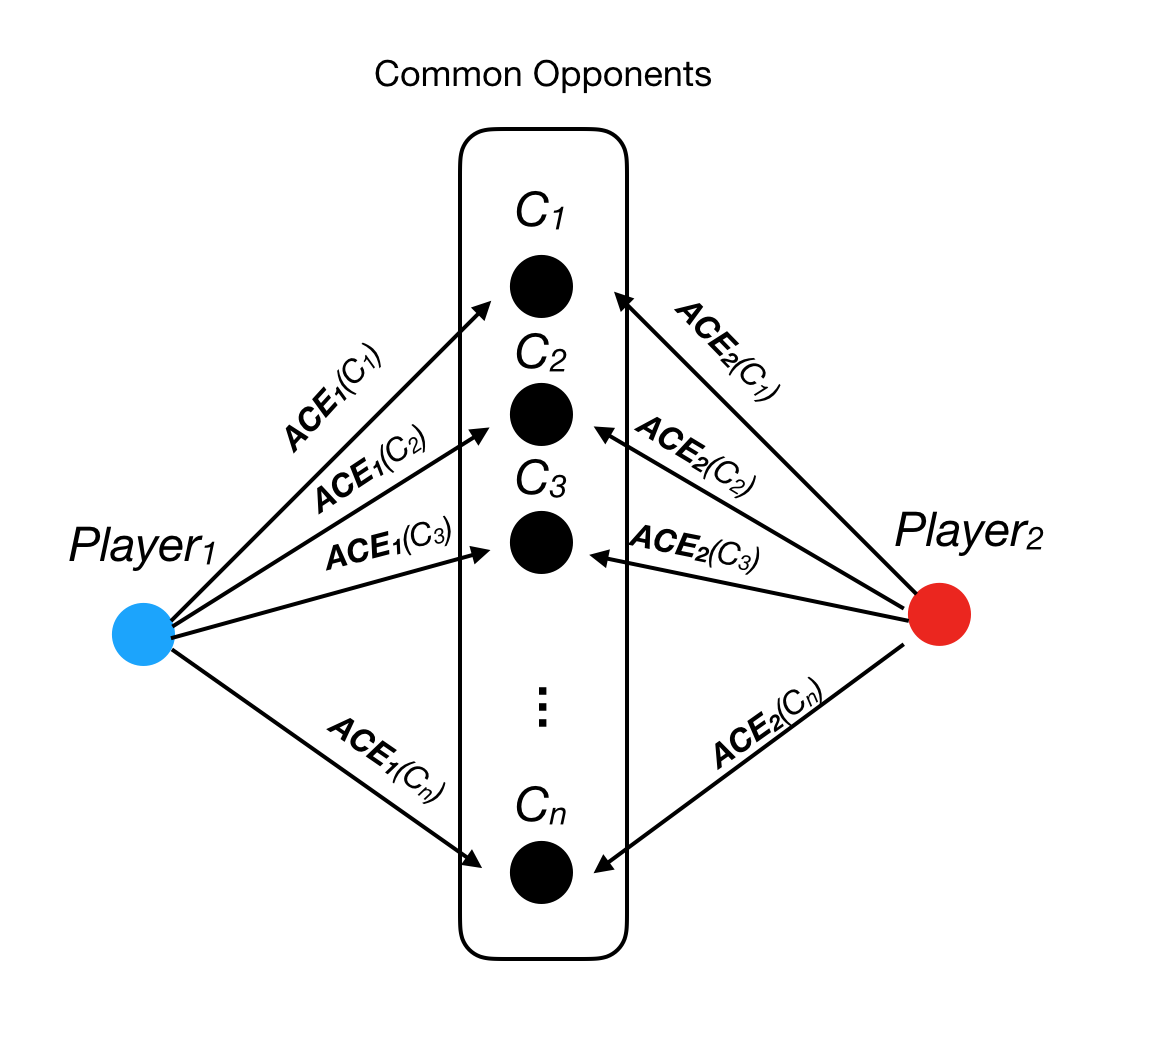
\includegraphics[width=0.8\textwidth]{CO}
  \label{fig:CO}
\end{figure}
As shown in Figure \ref{fig:CO}, common opponents are labeled as $C_1, C_2, ...C_n$. For Player $i \in \{1,2\}$, $ACE_i(C_j)$ is his/her average count of aces in all matches against common opponent $C_j$. We then take an average of these values to get $ACE_i$ for Player $i$: $$ACE_i = \frac{\Sigma_{j=0}^n ACE_i(C_j)}{n}$$
Lastly, applying the idea of difference variables, we create the feature ACE by finding the difference in performance on this feature between Player 1 and Player 2: $$ACE = ACE_1 - ACE_2$$. 
We can apply the same technique on other features too. The limitation of this method is apparent: it only works well when players actually have common opponents have played games with them before the queried match date. Hence, we need to think about how to handle edge cases.
\subsubsection{Edge Cases}
We have run into 2 edge cases: (1) when at least one of the players is new; (2) when two players do not have any common opponents. When (1) happens, it is necessarily the case that it suffers from (2) no common opponents as well; but the reverse is not true. \textbf{TODO}: add in what we decided to do
\subsection{Data Preparation}
\subsubsection{Data Source}
We obtain match-level data from Jeff Sackmann's Github repositories \cite{tennis_atp} \cite{tennis_charting}, with the Match Charting Project (MCP) providing set-level stats and results as well \cite{tennis_charting}. MCP is essentially a crowdsourced shot-by-shot professional tennis dataset, and it enables us to have a real-time lens into tennis matches. 
\subsubsection{Data Cleaning \& Transformation}
\textbf{TODO}: Things to talk about:
\begin{itemize}
\item Validations run on the datasets
\item How to detect and remove duplicates
\item Decision on dropping Davis Cup data (because team tourney might have different strategies, hence introducing biases)
\item How to merge two datasets together
\item (TODO for future work) Standardize features? 
\end{itemize}
\subsection{Feature List}
We present the list of extracted features in Table \ref{tab:features}. Note that all these features are difference variables unless otherwise noted. 
\begin{center}
\begin{table}[h]
    \begin{tabular}{  l | p{10cm} }
    \hline
    Feature  & Description \\ \hline
    \textbf{DURATION}  & Match duration in minutes (\textit{not difference}) \\ \hline
    \textbf{SAME\_HANDEDNESS}  & Tracking, on average, the frequency of facing opponents who have the same dominant hand \\ \hline
    \textbf{RANK}  & ATP rank \\ \hline
    \textbf{RANK\_PTS}  & ATP rank points \\ \hline
    \textbf{HEIGHT}  & Player height \\ \hline
    \textbf{FSP}  & First serve success percentage \\ \hline
    \textbf{ACE}  & Average number of aces per game \\ \hline
    \textbf{DF}  & Average number of double faults per game \\ \hline
    \textbf{BP\_FACED}  & Average number of break points faced per game \\ \hline
    \textbf{BP\_SAVED}  & Average number of break points saved per game \\ \hline
    \textbf{BPP}  & Break point saving percentage \\ \hline
    \textbf{SVGM}  & Average number of serve games \\ \hline
    \textbf{W1SP}  & Winning on first serve percentage \\ \hline
    \textbf{W2SP}  & Winning on second serve percentage \\ \hline
    \textbf{SVPT}  & Average number of serve points per game \\ \hline
    \end{tabular}
    \caption{Summary of extracted features}
    \label{tab:features}
    \end{table}
\end{center}
%----------------------------------------------------------------------------------------

%----------------------------------------------------------------------------------------
%	Section Preliminary Experiments
%----------------------------------------------------------------------------------------

\section{Preliminary Experiments}
As the team is still working on connecting the historical, match-level dataset with the real-time, set-level data sets, we ran some preliminary models fitting the two datasets separately instead. We use scikit-learn's implementation of the various models \cite{scikit-learn}.
\subsection{Historical, Match-level Dataset: Logistic Regression Model}
Applying a train-test split of 2:1, we trained a logistic regression model on 2/3 of all the ATP matches from 2012. Following the labelling from Section~\ref{sec:label}, we set $label = 1$ for all the matches with Player 1 being the Winner (notation-only), and then duplicated the entire dataset but swapped Player 1 and Player 2 and set $label = 0$, as well as inverted all difference features. \textbf{TODO}: might need more explanation? 

We achieved an impressive accuracy rate of 87.8\% just using the historical, match-level dataset with common opponent model and difference variables. 
\subsubsection{Error Analysis}
A preliminary error analysis was done to explore the relative importance of all the extracted features, and the results are shown in Table~\ref{tab:logreg}. Interestingly, we note that \textbf{RANK\_PTS} accounts for almost $20\%$ of the performance. 
\begin{center}
\begin{table}[h]
    \begin{tabular}{  l | l | l | p{5cm} }
    \hline
Order &     Accuracy Rate    &         Feature    &  Performance Difference \\ \hline
0    &    0.878170 &              \textbf{SVPT}  &      \\ \hline
1    &    0.878170 &        \textbf{SAME\_HANDEDNESS}  & 0.00\% \\ \hline
2    &    0.666483 &          \textbf{RANK\_PTS} & -21.17\% \\ \hline
3    &    0.657111 &              \textbf{RANK} & -0.94\% \\ \hline
4    &    0.660419 &            \textbf{HEIGHT} & 0.33\% \\ \hline
5    &    0.659868 &  \textbf{FSP} & -0.06\% \\ \hline
6    &    0.665932 &       \textbf{DURATION} &  0.61\% \\ \hline
7    &    0.661521 &                \textbf{DF} & -0.44\% \\ \hline
8    &    0.664278 &    \textbf{BPP} &  0.28\% \\ \hline
9    &    0.664829 &         \textbf{BP\_SAVED} &  0.06\% \\ \hline
10   &    0.665380 &          \textbf{BP\_FACED}  & 0.06\% \\ \hline
11   &    0.648842 &    \textbf{ACE} & -1.65\% \\ \hline
12   &    0.661521 &             \textbf{SVGM} & 1.27\% \\ \hline
13   &    0.659868 & \textbf{W2SP} & -0.17\% \\ \hline
    \end{tabular}
    \caption{Summary of extracted feature performance in the preliminary logistic regression model fitting on historical match-level data}
    \label{tab:logreg}
    \end{table}
\end{center}
\subsection{Historical, Match-level Dataset: Naive Bayes Classifier}
We also ran the data through a Gaussian-based Naive Bayes classifier, which showed an impressive 86.9\% accuracy rate (misclassifying 718 points out of 5496). As expected, it was also extremely fast. The impressive performance indicates that the extracted features might indeed be conditionally independent of each other, which is something we never thought of before, and look to explore in the next steps. On a first glance, it seems to suggest that given Player $i$ won the match, his/her performance on aces and rank point difference or double faults are indeed almost independent. We were surprised by the results, and more sanity check is needed before we put ourselves behind this. 
\subsection{Real-time, Set-level Dataset: Logistic Regression Model}
\textbf{TODO}
\subsection{Real-time, Set-level Dataset:  SVM}
\textbf{TODO}

%----------------------------------------------------------------------------------------
%	Section Next Steps
%----------------------------------------------------------------------------------------

\section{Next Steps}
The biggest next step is to connect the historical, match-level dataset with the real-time, set-level data set in order to conduct further experiments. We also plan to incorporate more sophisticated ideas on feature scaling in the context of tennis, such as \textbf{time discounting}, \textbf{surface weighting}, and the effect of fatigue and player injury. Moreover, we wanted to explore more interesting features such as \textbf{head-to-head results}, as well as to conduct \textbf{Principal Component Analysis} and \textbf{Feature Selection} to understand the inter-correlation between features, and which features are more predictive than others. Lastly, we plan to benchmark various machine learning models' performances, and to fine-tune the best them to achieve optimal performance. 
%----------------------------------------------------------------------------------------
%	Conclusion
%----------------------------------------------------------------------------------------
\section{Conclusion}
The use of common opponent model and difference variables already offer high predictive power in simple machine learning models such as logistic regression and Naive Bayes, and it's exciting to see with fine-tuning and more exploration and connecting datasets what we can achieve. It's also helpful to learn that ATP rank point difference between two players alone is already predictive of their likely match outcome. 

\appendix
%----------------------------------------------------------------------------------------
%	Section Contributions
%----------------------------------------------------------------------------------------

\section{Contributions}
\subsection{Yi Zhong}
\subsection{Yubo Tian}
\subsection{Yang "Eddie" Chen}
\begin{itemize}
\item Researched and reviewed relevant literature for applicable ideas, such as Clarke and Dyte \cite{Clarke2010} and O'Malley \cite{omalley} for difference variable, and Knottenbelt \cite{KNOTTENBELT20123820} for the common opponent model
\item Implemented the Common Opponent Model to look up players stats from common opponents
\item Generated ATP Match results for labels
\item Typsetted (\LaTeX) the project milestone report
\end{itemize}

\section{Appendix: Project Roadmap}
\begin{itemize}
\item \textbf{11/13 - 11/19}: Data cleaning
\item \textbf{11/20 - 11/26}: Preliminary experiements, building out more sophisticated ideas into models such as surface weighting, time decaying, fatigue, and injury
\item \textbf{11/27 - 12/03}: Continue fine-tuning models
\item \textbf{12/04 - 12/10}: Poster making
\item \textbf{12/11 - 12/15}: Poster presentation; final project write-up
\end{itemize}

\bibliographystyle{plain}
\bibliography{ref} 
\end{document}